
\section{Transformer}


\begin{frame}{Transformer: Self-Attention}
    
    \begin{itemizeSpaced}{2pt}
        \item Kind of seq-to-seq model used for machine translation; more parallelizable than seq-to-seq via abandoning RNNs and using only \textbf{self-attention} to generate sequence of \textit{contextual embeddings}.
        
    \end{itemizeSpaced}
    
    \begin{exampleBlock}{Example: Motivation for Self-Attention}
    {\large \emph{``The animal didn't cross the road because it was too tired."}}
    
    What does ``it" refer to? The road or animal?
    \end{exampleBlock}
    
    \begin{itemizeSpaced}{0pt}
        \pinkbox \textbf{Self-Attention} lets Transformer look at other words to \emph{bake in} their representations into the word ``it" while processing the input sequence.
        
        \item An \textbf{attention function} maps query and key-value pairs to output vector:
        
        \begin{itemizeSpaced}{0pt}
         
            \item Query matrix $Q$ rows signify which word to do self-attention (``it") on; Key matrix $K$ rows describe \emph{each} word in the sentence; Value matrix $V$ rows represent rest of the words (other than ``it"). 
            
            \item Final embedding of the word or \textbf{output} is a weighted sum of \textbf{value} vectors and softmax probabilities of the dot product between query and key vectors: 
            $$
            Attention \Big(Q, K, V \Big) = softmax \Bigg(\frac {QK^T} {\sqrt{d_k}} \Bigg) V
            $$
            
    \end{itemizeSpaced}
    
        \pinkbox Cements the values of words on which to focus while drowning out irrelevant words.
    \end{itemizeSpaced}
\end{frame}



\begin{frame}{Transformer: Multi-Head Attention}
    
    \begin{definitionBlock}{Definition: Multi-Head Attention}
        A \textbf{\alert{multi-head attention mechanism}} comprises of several self-attention heads. 
        
        Enables the Transformer to ``jointly attend to information from different representation subspaces at different positions." 
        
        A single attention head cannot do this because of averaging (Vaswani et al., 2017).
    \end{definitionBlock}
    
    \begin{itemizeSpaced}{4pt}
        \pinkbox Instead of calculating attention once, multi-head attention does (1) self attention many times in parallel on the projected dimensions, (2) concatenates the independent attention outputs, and (3) once again projects the result into the expected dimension to give a final value (Vaswani et al., 2017; Weng, 2018).
        
        \pinkbox More attention heads means Transformer can focus on different words; while encoding ``it", one attention head looks at ``the animal" while another focuses on ``tired" $\Rightarrow$ representation of ``it" includes some of all words. 
    \end{itemizeSpaced}
    
\end{frame}





\begin{frame}{Transformer: Positional Encodings}

    \begin{definitionBlock}{Definition: Positional Encoding}
        \normalsize 
        
        A \textbf{positional encoding} follows a specific, learned pattern to identify word position or the distance between words in the sequence (Alammar, 2018b). 
        
        $$
        \begin{array}{ll}
        \textit{PosEnc}_{\Large (\textit{pos}, 2i)} = \text{sin} \Bigg(\frac {\textit{pos}} {10000^{\Large \frac {2i} {d_{\textit{model}}} } }  \Bigg) \\
        \textit{PosEnc}_{\Large (\textit{pos}, 2i + 1)} = \text{cos} \Bigg(\frac {\textit{pos}} {10000^{\Large \frac {2i} {d_{\textit{model}}} } }  \Bigg)
        \end{array}
        $$
        where $\textit{pos} = $ a position, $i = $ a dimension.
    \end{definitionBlock}
    
    
    
    \begin{itemizeSpaced}{2pt}
        \pinkbox Transformer has no recurrence, so can't yet see \emph{order in the input sequence}. 
        
        \item Positional encodings act in place of recurrence mechanism to inject relative / absolute token position info so Transformer can see \emph{sentence order} when taking inputs.
        
        \begin{alertBlock}{Otherwise ...}
        ... the sentences ``I like dogs more than cats" and ``I like cats more than dogs" would encode the same meaning (Raviraja, 2019). 
        \end{alertBlock}
    \end{itemizeSpaced}
    
\end{frame}



% ERASE
\begin{frame}{Transformer: More Layers}

    \begin{itemizeSpaced}{3pt}
        \item \textbf{Positionwise feed-forward layer} is a kind of \textbf{feed-forward neural network (FFN)}, and is ``position-wise" since the FFN is applied to each position separately and identically.
        
        \item \textbf{Residual Connection: }a sub-layer in Encoder / Decoder stacks meant for harmonizing gradient optimization procedure.
        
        \item \textbf{Masked Multi-Head Attention: } key component in Decoder stack. Is attention with \textbf{masking} to prevent positions from attending to subsequent positions (while decoding word embedding $\overrightarrow{w_i}$, the Decoder is not allowed to see words  $\overrightarrow{w_{>i}}$ past position $i$, only words $\overrightarrow{w_{\leq i}}$, so no ``cheating" occurs (Ta-Chun, 2018). 
        
        \item \textbf{Encoder: } is bidirectional RNN that concatenates \emph{forward and backward} hidden states to get bidirectional context: $h_t = \Big \{ \overrightarrow{h}_t^T \; ; \; \overleftarrow{h}_t^T \Big\}^T , \: t=1,...,T_x$. \footnotemark 
        
        \item \textbf{Decoder: } neural network generates hidden states $s_t = \text{Decoder}\Big( s_{t-1}, y_{t-1}, c_t \Big)$ for times $t = 1,..., m$ \footnotemark  
        
    \end{itemizeSpaced}
    
    
    
    \footnotetext[8]{Note: arrows here denote the direction of the network rather than vector notation.}
    
    \footnotetext[9]{Context vector $c_t = \sum_{i=1}^n \alpha_{ti} \cdot h_i$ is a sum of the hidden states of the input sentence, weighted by alignment scores (same calculation as in the seq-to-seq model)}
    
\end{frame}


\begin{frame}{Transformer: Encoder and Decoder Stack in Detail}

    \begin{itemizeSpaced}{2pt}
        \item Encoder and Decoder are each composed of $N$ identical \textbf{layers} or \textbf{stack}.
    
        \item A \textbf{residual connection layer} then layer normalization surround each sub-layer.  
    
    
    \end{itemizeSpaced}
    
    
    \begin{figure}[h]
    \vspace{-10pt}
    \centering
    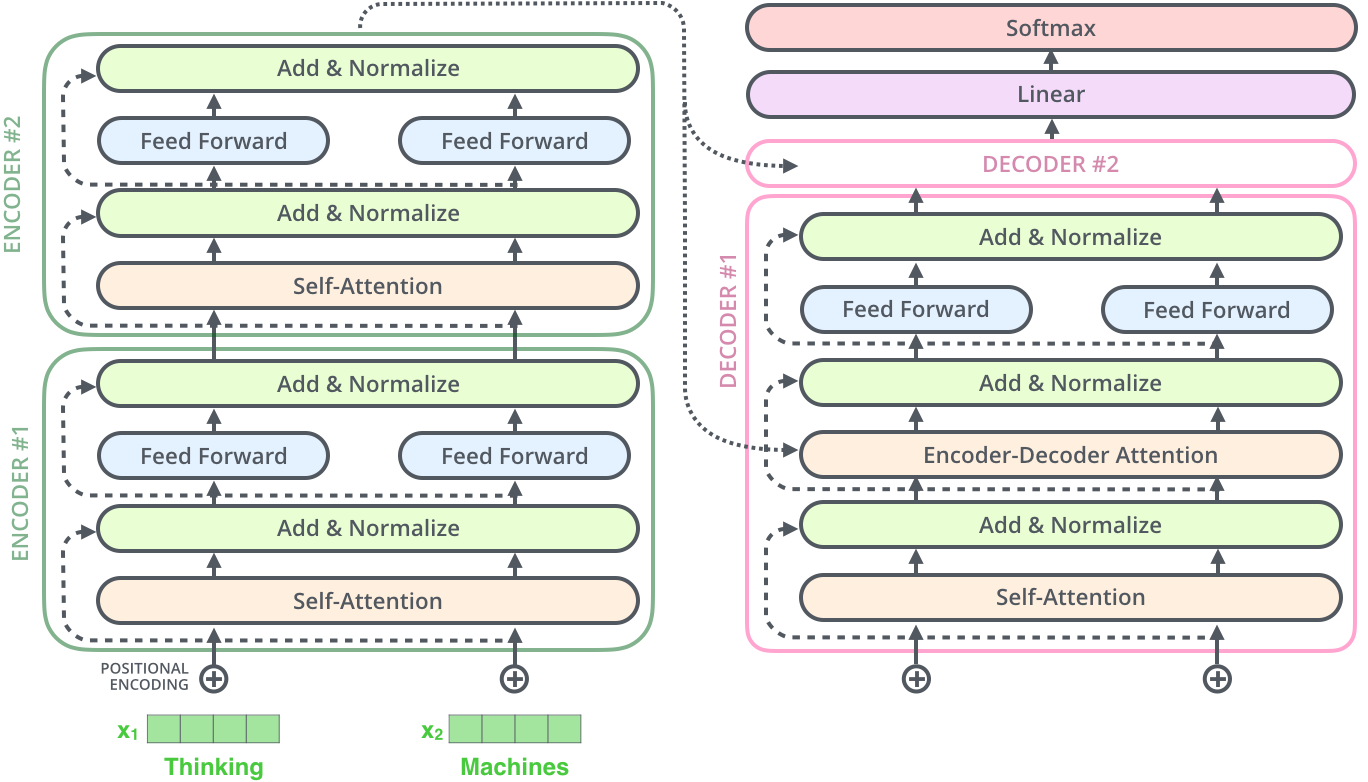
\includegraphics[width=0.9\textwidth]{imgs/encoderDecoderLayersDetailed.png}
    \vspace{-10pt}
    \caption{\linespread{0.4} \footnotesize Encoder layer contains: (1) Multi-head attention, (2) Position-wise feed forward layer. Decoder layer contains: (1) Masked multi-head attention, (2) Encoder-Decoder attention, (3) Position-wise feed forward layer. From \emph{The Illustrated Transformer}, by Alammar, 2018. \url{https://jalammar.github.io/illustrated-transformer/}. Copyright 2018 by Alammar. }
    \vspace{-5pt}
    \label{fig:encDecLayersDetailed}
    \end{figure}
    
\end{frame}





% ERASE
\begin{frame}{Transformer: How Do We Predict a Word?}
    \large 
    
    Generally ...
    
    Decoder stack $\Rightarrow$ Linear layer $\Rightarrow$ Softmax layer. 

    \begin{itemizeSpaced}{7pt}
        \item \textbf{Linear Layer} neural network projects Decoder's float vector to larger dimension ``logit vector" (each cell holds a score corresponding to each unique vocabulary word.)
    
        \item \textbf{Softmax Layer} then converts the Linear Layer's scores into probabilities via the softmax function. 
    \end{itemizeSpaced}

    \textbf{To find the predicted word: } the cell with highest probability is chosen $\Rightarrow$ its word is the ``predicted" word. 

    
\end{frame}